\documentclass[usenames,dvipsnames,8pt,aspectratio=169]{beamer}
\usepackage{amsmath,amsfonts,amssymb}
\usepackage{mathtools}
\usepackage{etex} %for Windows
\usepackage[utf8]{inputenc}
\usepackage[english, russian]{babel} 
%\usepackage{microtype}			% Better interword spacing and additional kerning.
\usepackage{ellipsis}			% Adjusted space with \dots between two words.
\usepackage{graphicx}
\usepackage{pstricks}

\usepackage{xcolor}


\usepackage{changepage}

\usepackage{algorithm}
\usepackage{algpseudocode}
%\usepackage[]{algorithm2e}
%\usepackage{algorithmic}

%\usepackage{tcolorbox}


\usepackage{caption}
\usepackage{subcaption}
%\usepackage{stackengine}


\usepackage{tikz}
\usetikzlibrary{tikzmark,calc}
\usetikzlibrary{positioning, backgrounds}
\usetikzlibrary{arrows, chains, matrix, scopes, patterns, shapes, fit}
\usetikzlibrary{mindmap,trees,shadows}
\usetikzlibrary{decorations.pathreplacing}
%\usetikzlibrary{crypto.symbols}

\usepackage{pgfplots}

\pgfmathdeclarefunction{gauss}{2}{%
	\pgfmathparse{1/(#2*sqrt(2*pi))*exp(-((x-#1)^2)/(2*#2^2))}%
}


\tikzset{
	invisible/.style={opacity=0},
	visible on/.style={alt={#1{}{invisible}}},
	alt/.code args={<#1>#2#3}{%
		\alt<#1>{\pgfkeysalso{#2}}{\pgfkeysalso{#3}} % \pgfkeysalso doesn't change the path
	},
}

\newcommand\strikeout[2][]{%
	\begin{tabular}[b]{@{}c@{}} 
		\makebox(0,0)[cb]{{#1}} \\[-0.2\normalbaselineskip]
		\rlap{\color{Orange}\rule[0.5ex]{\widthof{#2}}{1.5pt}}#2
\end{tabular}}

\newcommand\Fontvi{\fontsize{11}{13.2}\selectfont}

\usepackage{listings} % for C++ code

\usepackage{braket}
%\usepackage[braket, qm]{qcircuit}



\usepackage[T1]{fontenc}
%\usepackage[sfdefault,scaled=.85]{FiraSans}
%\usepackage{newtxsf}
%\usepackage[nomap]{FiraMono}





\usefonttheme[onlymath]{serif}
\renewcommand\sfdefault{cmbr}

\renewcommand{\bfdefault}{sb}

\definecolor{CharCoalDark}{RGB}{13, 16, 19}
\definecolor{Orange}{RGB}{255, 165,0}
\definecolor{DarkOrange}{RGB}{255, 165,0}
\definecolor{LightSalmon}{RGB}{255, 160, 122}
\definecolor{LeafGreen}{RGB}{34, 139,  34}
\definecolor{Coral}{RGB}{255, 127, 80}
\definecolor{DarkTurquoise}{RGB}{0, 206, 209}

%\newtheorem{defRus}{Определение}
%\newtheorem{thmRus}{Теорема}
%s\newtheorem{corRus}{Следствие}


\setbeamercolor{background canvas}{bg=CharCoalDark}

\setbeamerfont{title}{series=\bfseries}
\setbeamercolor{title}{fg=Orange}
\setbeamercolor{section in toc}{fg=white}
\setbeamercolor{frametitle}{fg=Orange}
\setbeamercolor{normal text}{fg=white}
%\setbeamercolor{normal text}{fontsize=12pt}
\setbeamercolor{itemize item}{fg=Orange}
\setbeamercolor{enumerate item}{fg=Orange}
\setbeamercolor{enumerate item item}{fg=Orange}
\setbeamercolor{itemize item item}{fg=Orange}
\setbeamercolor{enumerate item}{fg=Orange}
\setbeamercolor{block title}{bg=DarkOrange,fg=white}
\setbeamerfont{block title}{series=\bfseries}

\setbeamertemplate{itemize item}[circle]
\setbeamertemplate{eumerate subitem}{\color{Orange}[$\checkmark$]}
\setbeamertemplate{itemize subitem}{\color{Orange}\Large$\textbullet$}
\setbeamertemplate{itemize subitem}{\color{Orange} \tiny $\blacksquare$}

% footnote without a marker
\newcommand\blfootnote[1]{%
	\begingroup
	\renewcommand\footnoterule{}
	\renewcommand\thefootnote{}\footnote{#1}%
	\addtocounter{footnote}{-1}%
	\endgroup
}

\newcommand*{\Scale}[2][4]{\scalebox{#1}{\ensuremath{#2}}}%

\newcommand\Item[1][]{%
	\ifx\relax#1\relax  \item \else \item[#1] \fi
	\abovedisplayskip=0pt\abovedisplayshortskip=0pt~\vspace*{-\baselineskip}}

\pgfdeclareradialshading{ring}{\pgfpoint{0cm}{0cm}}%
{rgb(0cm)=(1,1,1);
	rgb(0.7cm)=(1,1,1);
	rgb(0.719cm)=(1,1,1);
	rgb(0.72cm)=(0.975,0,0);
	rgb(0.9cm)=(1,1,1)}

\addtobeamertemplate{footline}{%
	\setlength\unitlength{1ex}%
	\begin{picture}(0,0) 
	% \put{} defines the position of the frame
	\put(155,0){\makebox(0,0)[bl]{
			%
\includegraphics[scale=0.65]{white_square}
			%
\includegraphics[scale=0.65]{dark_square}
			
\includegraphics[scale=0.65]{grey_circle}
	}}%
	\end{picture}%
}{}


\usepackage[absolute,overlay]{textpos} %to clip to a corner
\newcommand\FrameText[1]{%
	\begin{textblock*}{\paperwidth}(\textwidth-35pt, 10 pt)
		\raggedright #1\hspace{.5em}
\end{textblock*}}

\makeatletter
\let\save@measuring@true\measuring@true
\def\measuring@true{%
	\save@measuring@true
	\def\beamer@sortzero##1{\beamer@ifnextcharospec{\beamer@sortzeroread{##1}}{}}%
	\def\beamer@sortzeroread##1<##2>{}%
	\def\beamer@finalnospec{}%
}
\makeatother

\AtBeginSection[]
{
	\begin{frame}<beamer>
		\frametitle{Outline}
		\tableofcontents[currentsection]
	\end{frame}
}


\title{Лекция №6 \\[10pt]
	Часть 1. Шифрование с аутентификацией. Определение }

\date{ Елена Киршанова \\  \textbf{Курс ``Основы криптографии''} \\  }



\setbeamertemplate{navigation symbols}{} %removes navigation

% proper highlightling of a code-snippet
\lstset{language=C++,
	keywordstyle=\color{magenta},
	stringstyle=\color{Goldenrod},
	commentstyle=\color{gray},
	breaklines=false,
	%morecomment=[l][\color{magenta}]{\#}
}

%\setlength{\parskip}{8pt}
% ==================================================================
% Definitions for this paper
% ==================================================================
\mathchardef\hyphen="2D

\usepackage{multirow}
\usepackage{multicol} % For multiple coloumn environments
%\usepackage{stmaryrd} % For set brackets
% \setlength{\columnsep}{15pt} % Defining the coloumn seperation
% \setlength{\columnseprule}{1pt} % Place a line between coloumns
% \newcommand{\tab}{\hspace*{2em}}

%subscripts

\newcommand*\SmallTextScript[2]{{\mathchoice{\displaystyle #2}
		{\textstyle #2}%dito
		{\scalebox{#1}{\ensuremath{\scriptstyle #2}}}%
		{\scalebox{#1}{\ensuremath{\scriptscriptstyle #2}}}%
}}


% ADVERSARIES AND SUCH
\newcommand*{\poly}{\ensuremath{\mathrm{poly}}}
\newcommand*{\eps}{\ensuremath{\varepsilon}}
\newcommand*{\alg}{\ensuremath{\mathcal{A}}}

% GROUPS/DISTRIBUTIONS/SETS/LISTS
\newcommand{\N}{{{\mathbb N}}}
\newcommand{\Z}{{{\mathbb Z}}}
\newcommand*{\IZ}{\ensuremath{\mathbb{Z}}}
\newcommand*{\IN}{\ensuremath{\mathbb{N}}}
\newcommand*{\IQ}{\ensuremath{\mathbb{Q}}}
\newcommand{\R}{{{\mathbb R}}}
\newcommand*{\IR}{{{\mathbb R}}}
\newcommand{\Zp}{\ints_p} % Integers modulo p
\newcommand{\Zq}{\ints_q} % Integers modulo q
\newcommand{\Zn}{\ints_N} % Integers modulo N
\newcommand{\F}{\ensuremath{\mathbb{F}}}
\newcommand{\CC}{\ensuremath{\mathbb{C}}}

\newcommand{\GF}{\ensuremath{\mathbb{F}_2}}
\newcommand{\GFn}{\ensuremath{\mathbb{F}^n_2}}

%%% ALGORITHMS/PROCEDURES %%%
\newcommand{\Dec}{\textsf{Dec}}
\newcommand{\Enc}{\textsf{Enc}}
\newcommand{\KeyGen}{\textsf{KeyGen}}
\newcommand{\Gen}{\textsf{Gen}}
\newcommand{\sk}{\textsf{sk}}
\newcommand{\pk}{\textsf{pk}}
\newcommand{\vk}{\textsf{vk}}
\newcommand{\mesS}{\ensuremath{\mathcal{M}}}
\newcommand{\keyS}{\ensuremath{\mathcal{K}}}
\newcommand{\cipS}{\ensuremath{\mathcal{C}}}
\newcommand{\tagS}{\ensuremath{\mathcal{T}}}
\newcommand{\mactag}{\textsf{tag}}
\newcommand{\Hash}{\ensuremath{\mathcal{H}}}
\newcommand{\EID}{\ensuremath{\mathtt{EphID}}}


\newcommand{\adv}{\ensuremath{\mathcal{A}}}

\newcommand{\LWE}{\mathsf{LWE}}
\newcommand{\DCP}{\mathsf{DCP}}
\newcommand{\EDCP}{\mathsf{EDCP}}
\newcommand{\UEDCP}{\mathsf{U \text{-} EDCP}}
\newcommand{\GEDCP}{\mathsf{G \text{-} EDCP}}



%% Landau and proba
\newcommand{\bigO}{\mathcal{O}}
\newcommand*{\OLandau}{\bigO}
\newcommand*{\WLandau}{\Omega}
\newcommand*{\xOLandau}{\widetilde{\OLandau}}
\newcommand*{\xWLandau}{\widetilde{\WLandau}}
\newcommand*{\TLandau}{\Theta}
\newcommand*{\xTLandau}{\widetilde{\TLandau}}
\newcommand{\smallo}{o} %technically, an omicron
\newcommand{\wLandau}{\omega}
\newcommand{\negl}{\mathrm{negl}}
\newcommand*\PROB\Pr 
\DeclareMathOperator*{\EXPECT}{\mathbb{E}}
\DeclareMathOperator*{\VARIANCE}{\mathbb{V}}
\DeclareMathOperator*{\LOGBIAS}{\mathbb{LB}}

\newcommand{\supp}{\ensuremath{\mathsf{sup}}}
\newcommand{\Distr}{\ensuremath{\mathcal{D}}}

% Lattices

% \newcommand{\coset}{\Lambda} % Lambda Lattice
% \newcommand{\cosetPerp}{\Lambda^{\bot}} % Lambda_Perp Lattice
% \newcommand{\gadget}{\textbf{G}} %Gaget matrix
% \newcommand{\mes}{\textbf{m}} %message vector
% \newcommand{\AMat}{\textbf{A}} %A matrices
% \newcommand{\BMat}{\textbf{B}} %B matrices
% \newcommand{\RMat}{\textbf{R}} %R matrices
% \newcommand{\HMat}{\textbf{H}} %H matrices
% \newcommand{\XMat}{\textbf{X}} %H matrices
% \newcommand{\mbar}{\bar{m}} %mBar dimension
% % \newcommand{\gauss}{\mathcal{D}} % gaussian distribution
% \newcommand{\Id}{\textbf{I}} % Identity matrix
% \newcommand{\er}{\textbf{e}} % gaussian distr. vectors
% % \newcommand{\cipher}{\textit{c}} % ciphertext
% \newcommand{\Olwe}{\mathcal{O}_{\textsf{LWE}}} %LWE oracle
% \newcommand{\OSample}{\mathcal{O}_{Sample}} %LWE oracle
% \newcommand{\SigmaB}{\boldsymbol{\Sigma}} %semi-deifinite matrix Sigma%
% % \newcommand{\mods}{\text{ mod}}


%Vectors and Matrices

\newcommand{\AMat}{\mathbf{A}} %A matrices
\newcommand{\BMat}{\mathbf{B}} %B matrices
\newcommand{\DMat}{\mathbf{D}} %Diagonal


\newcommand{\HMat}{\ensuremath{\mathbf{H}}}
\newcommand{\QMat}{\ensuremath{\mathbf{Q}}}
\newcommand{\Id}{\ensuremath{\mathbf{I}}}
\newcommand{\ZeroM}{\textbf{0}} % Zero matrix

\newcommand{\avec}{\ensuremath{\mathbf{a}}}
\newcommand{\bvec}{\ensuremath{\mathbf{b}}}
\newcommand{\cvec}{\ensuremath{\mathbf{c}}}
\newcommand{\evec}{\ensuremath{\mathbf{e}}}
\newcommand{\rvec}{\ensuremath{\mathbf{r}}}
\newcommand{\svec}{\ensuremath{\mathbf{s}}}
\newcommand{\tvec}{\ensuremath{\mathbf{t}}}
\newcommand{\vvec}{\ensuremath{\mathbf{v}}}
\newcommand{\zvec}{\ensuremath{\mathbf{z}}}
\newcommand{\xvec}{\ensuremath{\mathbf{x}}}
\newcommand{\yvec}{\ensuremath{\mathbf{y}}}
\newcommand{\uvec}{\ensuremath{\mathbf{u}}}
\newcommand{\zerovec}{\ensuremath{\mathbf{0}}}

\newcommand{\nth}{^{\mathrm{th}}}
\newcommand{\nd}{^{\mathrm{nd}}}

\newcommand{\RepMMT}{\ensuremath{\mathcal{R}_{\protect\SmallTextScript{0.70}{\texttt{MMT}}}}}
\newcommand{\RepBJMM}{\ensuremath{\mathcal{R}_{\protect\SmallTextScript{0.70}{\texttt{BJMM}}}}}
\newcommand{\XOR}{\ensuremath{\mathtt{3XOR}}}


% % % % % \newcommand{\mb}[1]{\mathbf{#1}} % does not compile otherwise
%%% Removed by Gotti; this is just asking to screw up with packages that (properly) define \mb (mathbold)

% \newcommand{\bL}{\|\bvec_1\|} % b1 length that appears way too often
% \newcommand{\dL}{\|\dvec_1\|} % b1 length that appears way too oftend

%Norms and Scalar products

\newcommand*\abs[1]{\left\lvert#1\right\rvert}
\newcommand*\norm[1]{\left\lVert#1\right\rVert}
\newcommand*\normalabs[1]{\lvert#1\rvert} 
\newcommand*\normalnorm[1]{\lVert#1\rVert}
\newcommand*\bignorm[1]{\bigl\lVert#1\bigr\rVert}
\newcommand*\bigabs[1]{\bigl\lvert#1\bigr\rvert}
\newcommand*\Bigabs[1]{\Bigl\lvert#1\Bigr\rvert}
\newcommand*{\ScProd}[2]{\ensuremath{\langle#1\mathbin{,}#2\rangle}} %Scalar Product
% \newcommand*{\ScProd}[2]{\ensuremath{\langle#1 \:{,}\:#2\rangle}} %Scalar Product
\newcommand*{\bigScProd}[2]{\ensuremath{\bigl\langle#1\mathbin{,}#2\bigr\rangle}} %Scalar Product
\newcommand*{\BigScProd}[2]{\ensuremath{\Bigl\langle#1\mathbin{,}#2\Bigr\rangle}} %Scalar Product
\newcommand{\dist}{\ensuremath{\text{dist}}}


%Some other math operators

\DeclareMathOperator{\Span}{Span} %span of vectors
\DeclareMathOperator{\vol}{\mathrm{vol}} %volume
\DeclareMathOperator{\LW}{LambertW} %Lambert W function
\DeclareMathOperator{\SD}{SD}
\DeclareMathOperator{\gradient}{grad}
\DeclareMathOperator{\TRACE}{Tr}
\newcommand*{\dDR}{\mathrm{d}} %de-Rham-Differential (the d in dx, dy, dz and so on)


%Lists
\renewcommand{\L}{\ensuremath{\mathcal{L}}}

\renewcommand{\P}{\ensuremath{\mathcal{P}}}

\newcommand*{\Lout}{\ensuremath{\L_{\mkern-0.5mu\protect\SmallTextScript{0.85}{\textup{out}}}}}
\newcommand*{\Sout}{\ensuremath{S_{\mkern-0.5mu\protect\SmallTextScript{0.85}{\textup{out}}}}}
\newcommand{\wt}{\ensuremath{\mathit{wt}}}


\newcommand*{\softO}{\widetilde{\bigO}}

\newcommand{\const}{\mathsf{c}} 


\newcommand{\transpose}{\mkern0.7mu^{\mathsf{ t}}}

%proper overline reduced by 1.5mu
\newcommand{\overbar}[1]{\mkern 1.5mu\overline{\mkern-1.5mu#1\mkern-1.5mu}\mkern 1.5mu}

\DeclareMathOperator{\erf}{erf} %error function
\DeclareMathOperator{\erfc}{erfc} %complementary error function
\newcommand{\Er}{\ensuremath{\mathrm{Er}}} %complementary error function


% LATTICES

\newcommand{\Lat}{\ensuremath{\mathcal{L}}}
\newcommand*{\Sphere}[1]{\ensuremath{\mathsf{S}^{#1}}}
%\DeclareMathOperator{\Conf}{Conf}
\newcommand{\Conf}{\mathcal{C}}

%Thick line for table
\setlength{\doublerulesep}{0pt}
\newcommand{\thickline}{\hline\hline\hline}


%circled text
\newcommand*\circled[1]{\tikz[baseline=(char.base)]{
    \node[shape=circle,draw,inner sep=0.3 pt] (char) {\scriptsize #1};}}


%Fix Algorithmicx package
\def\NoNumber#1{{\def\alglinenumber##1{}\State #1}\addtocounter{ALG@line}{-1}}

%For comments
\newcommand{\GColor}{ForestGreen}  %Damiens' color
\newcommand{\EColor}{MidnightBlue} %Elena's color

\newcommand*{\E}[1]{{\color{\EColor} #1} } 
\newcommand*{\G}[1]{{\color{\GColor} #1} } 

%Proper limit with the subscript underneath
% \newcommand{\Lim}[1]{\raisebox{0.5ex}{\scalebox{0.8}{$\displaystyle \lim_{#1}\;$}}}


%TIKZ dense dotted pattern

\pgfdeclarepatternformonly{my dots}{\pgfqpoint{-1pt}{-1pt}}{\pgfqpoint{2.0pt}{2.0pt}}{\pgfqpoint{2pt}{2pt}}%
{
	\pgfpathcircle{\pgfqpoint{0pt}{0pt}}{.35pt}
	\pgfpathcircle{\pgfqpoint{1pt}{1pt}}{.35pt}
	\pgfusepath{fill}
}


\tikzset{
	master/.style={
		execute at end picture={
			\coordinate (lower right) at (current bounding box.south east);
			\coordinate (upper left) at (current bounding box.north west);
		}
	},
	slave/.style={
		execute at end picture={
			\pgfresetboundingbox
			\path  (lower right)rectangle (upper left) ;
		}
	}
} %all defs

\newcommand{\AxisRotator}[1][rotate=0]{%
	\tikz [x=0.5cm,y=1.9cm,line width=.2ex,-stealth,#1] \draw[color=Orange] (0,0) arc (-150:150:2 and 1);%
}

\begin{document}
	
\begin{frame}
	\titlepage
\end{frame}

\begin{frame}{Agenda}
	\Large 
	До сегодняшнего дня 
	\begin{itemize}
		\item Конфиденциальность (Симметрическое шифрование)
		\item Целостность (MAC, HMAC)
	\end{itemize}
	\vspace{20pt}
	Эти примитивы защищают данные от {\color{Orange} пассивного (eavesdropping) злоумышленника}\\
	 
	\vspace{20pt}
	В этой лекции: \\
	Безопасность данных относительно {\color{Orange} активного (tampering)  \\ злоумышленника}\\[10pt]
	\LARGE Шифрование с аутентификацией (Authenticated Encryption)

\end{frame}

\begin{frame}{Шифрование с аутентификацией: определение}
\Large

{\color{Orange}{Шифрование с аутентификацией (AE)}} состоит из трех ppt алгоритмов
\begin{itemize}
	\itemsep 10pt
	\item Генерация ключа: $\KeyGen(1^\lambda): k \leftarrow \keyS$
	\item Шифрование: $\Enc: \keyS \times \mesS \times \nonceS \rightarrow \cipS$
	\item Дешифрование:  $\Dec: \keyS \times \cipS  \times \nonceS \rightarrow \mesS \cup \{\bot\}$
\end{itemize}
\vspace{15pt}
$\keyS$ - мн-во ключей, $\mesS$ - мн-во открытых текстов, $\cipS$ - мн-во шифр-текстов,  \\ $\nonceS$ - мн-во {\color{Orange} нонсов}. \\[10pt]


НОВОЕ: $\{\bot\}$ -- шифр-текст отклонен \\[10pt]


{\color{Orange} Нонсе (nonce)} = ``number that can only be used once'' \\[5pt]
Нонс может быть предсказуем, но он не должен быть использован \\ {\color{Orange} дважны} для одного ключа. \\[5pt]
%Пример: значения, полученные из IV в различных режимах симм. шифрования. 

\end{frame}

\begin{frame}{Корректность, безопасность шифрования с аутентификацией }
\Large
{\color{Orange}{Шифрование с аутентификацией (AE)}} состоит из трех ppt алгоритмов
\begin{itemize}
	\itemsep 10pt
	\item Генерация ключа: $\KeyGen(1^\lambda): k \leftarrow \keyS$
	\item Шифрование: $\Enc: \keyS \times \mesS \times \nonceS \rightarrow \cipS$
	\item Дешифрование:  $\Dec: \keyS \times \cipS  \times \nonceS \rightarrow \mesS \cup \{\bot\}$
\end{itemize}

\vspace{15pt}
{\color{Orange}{Корректность:}} $\forall m, \forall k, \forall n:$ $\Dec(k, \Enc(k, m,n), n) = m$

\vspace{15pt}
{\color{Orange}{Безопасность (неформально):}}
\begin{itemize}
	\itemsep 10pt
	\item $\Enc(k, m_0, n)$ неотличимо от $\Enc(k, m_1, n)$ $\forall m_0 != m_1$ (без знания $k$) 
	\item  Эффективный злоумышленник не в состоянии сформировать \\ шифр-текст, которые не дешифруется в $\{\bot\}$.
\end{itemize}

\end{frame}

\begin{frame}{Безопасность шифрования с аутентификацией}
	\Large
	Шифрование с аутентификацией обеспечивает
	\begin{itemize}
		\itemsep 10pt
		\item {\color{Orange}Аутентификацию:} Если $\Dec(k, c, n)!=\{\bot\}$, получатель знает, что сообщение пришло от того, кто знает $k$
		\pause
		\item {\color{Orange}AE $\implies$ стойкость относительно атаки на выбранный шифр-текст} 
	\end{itemize}

\vspace{15pt}
В  атаке на выбранный шифр-текст (Chosen Ciphertext Attack, CCA)  злоумышленник может
\begin{itemize}
	\item получить шифрования сообщений по своему выбору
	\item запросить дешифрование {\color{Orange}{любого}} шифр-текста по своему \\ выбору кроме кроме одного фиксированного чалленджа  $c$
\end{itemize}
%\vfill
%\centering
%\color{Orange} A CCA adversary is a very powerful adversary. \\
%Why does it capture real life attacks?
\end{frame}

\begin{frame}{Атака на выбранный открытый текст/ Chosen Plaintext Attack(CPA) (лекция №3)}
\large
\begin{center}
	
	\begin{tabular}{c c c}
		{\color{Orange} Челленджер $\mathcal{C}$ } & & {\color{Orange} Атакующий $\mathcal{A}$ }\\ [5pt]
		$k \leftarrow \KeyGen(1^\lambda)$ & $\xrightarrow{\quad \Huge \lambda \quad}$  &\\[5pt]
		$b \xleftarrow{\$} \{0,1\}  $& &\\ [5pt]
		& $\xleftarrow{\; \Huge m_{0, i}, m_{1, i}  \;}$  &$m_{0, i}, m_{1,i} \leftarrow \mesS $\\ [5pt]
		
		$c_i \leftarrow \Enc(k, m_{b, i})$ &  &\\ [5pt]
		& $\xrightarrow{\quad c_i \quad}$ & \\ [5pt]
		& $\xleftarrow{\quad \hat{b} \quad}$ & \\ [5pt]
	\end{tabular}
	\begin{tikzpicture}[overlay]
	\draw[fill=none, draw=white, opacity=0.5] (-8.3,-2.3) rectangle (-5.0,2.7); 
	\draw[fill=none, draw=white, opacity=0.5] (-3.0,-2.3) rectangle (0.0,2.7); 
	\node at (-3.8, -0.1) {\AxisRotator};
	\end{tikzpicture}
\end{center}

\vspace{5pt}
$\mathtt{W_{\Pi, \adv}}$ -- событие $b == \hat{b}$. \\ [4pt]
$\mathtt{CPAAdv} = \abs{\Pr[\mathtt{W_{\Pi, \adv}}] - \frac{1}{2}}$ --выигрыш  $\adv$. \\ [4pt]
\color{Orange} Шифр-схема $\Pi$ CPA безопасна, если для любого ppt $\adv:$  $\mathtt{CPAAdv} = \negl(\lambda).$
\end{frame}

\begin{frame}{Атака на выбранный шифр-текст/ Chosen Ciphertext Attack(CCA) }
	\large
	\begin{center}
		
		\begin{tabular}{c c c}
			{\color{Orange} Челленджер $\mathcal{C}$ } & & {\color{Orange} Атакующий $\mathcal{A}$ }\\ [5pt]
			$k \leftarrow \KeyGen(1^\lambda)$ & $\xrightarrow{\quad \Huge \lambda \quad}$  &\\[5pt]
			$b \xleftarrow{\$} \{0,1\}  $& &\\ [5pt]
			& $\xleftarrow{\; \Huge m_{0, i}, m_{1, i}  \;}$  &$m_{0, i}, m_{1,i} \leftarrow \mesS $\\ [2pt]
			
			$c_i \leftarrow \Enc(k, m_{b, i})$ &  &\\ [2pt]
			$C = C \cup \{c_i\} $ & $\xrightarrow{\quad c_i \quad}$  &\\ [8pt]
			
			& $\xleftarrow{\; c_j \notin C   \;}$  &\\ [5pt]
			$\hat{m_j} \leftarrow \Dec(k, c_{j})$  &  $\xrightarrow{\quad c_i \quad}$ & \\[2pt]
			& $\xleftarrow{\quad \hat{b} \quad}$ & \\ [5pt]
		\end{tabular}
		\begin{tikzpicture}[overlay]
		\draw[fill=none, draw=white, opacity=0.5] (-8.3,-2.5) rectangle (-5.0,3.2); 
		\draw[fill=none, draw=white, opacity=0.5] (-3.0,-2.5) rectangle (0.0,3.2); 
		\node at (-3.8, -0.1) {\AxisRotator};
		\end{tikzpicture}
	\end{center}
	
	\vspace{-5pt}
	$\mathtt{W_{\Pi, \adv}}$ -- событие $b == \hat{b}$. \\ [4pt]
	$\mathtt{CCAAdv} = \abs{\Pr[\mathtt{W_{\Pi, \adv}}] - \frac{1}{2}}$ --выигрыш  $\adv$. \\ [4pt]
	\color{Orange} Шифр-схема $\Pi$ CCA безопасна, если для любого ppt $\adv:$  $\mathtt{CCAAdv} = \negl(\lambda).$
\end{frame}

\begin{frame}{Пример of CCA атаки (IPSec, упрощенна версия)}
\Large 
Пусть $\Enc$ шифрование в режиме CTR \\
Сообщение $m$ состоит из хэдера ``Боб'+текст сообщения

\LARGE
	\begin{center}
		\begin{tabular}{c c c c c}
			Алиса &     &Почтовый сервер  & &Боб\\
			$k$ & {\huge $\xrightarrow{c \;= \Enc(k,\, m = \text{Боб||...})}$ }  &  $k$ & $\xrightarrow{\hspace{10pt}m\hspace{10pt}}$ & \pause\\[8pt] 
			&  $\xrightarrow{\Huge \hspace{1em}c\hspace{1em}}$ Ева  $\xrightarrow{\hspace{1em}\hat{c}\hspace{1em}}$  & & & \\
		\end{tabular}
	\end{center}

\Large
Положим $\mathtt{len}$(``Боб'') $==$  $\mathtt{len}$(``Ева'') $==$ длине блока.
\vspace{15pt}
\begin{columns}
	\begin{column}{0.4\linewidth}
		\begin{figure}
		\hspace{-30pt}	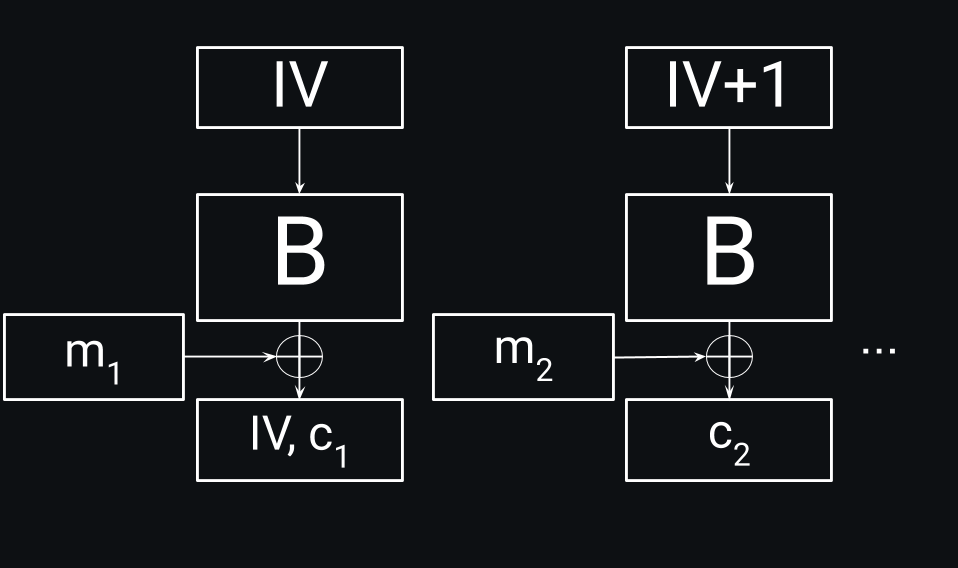
\includegraphics[width=0.9\linewidth]{CTR}
		\end{figure}
	\end{column}
	\begin{column}{0.4\linewidth}
{
\hspace{-50pt}
{\color{Orange} $\hat{c_1} = c_1 \oplus $[``Боб''] $\oplus$ [``Ева''] } \\[5pt]
\hspace{-50pt}Оставшиеся блоки $\hat{c}$ равные$c$.\\[5pt]
\hspace{-50pt}Ева узнает $m$, запрашивая $\Dec(\hat{c})$.
}
	\end{column}

\end{columns}
\end{frame}

%\begin{frame}{Construction of AE}
%\Large 
%\centering
%{\color{Orange} AE = Secure Encryption + Secure Mac} \\[10pt]
%
%Two keys: Encryption key $k_E$, MAC key $K_M$ \\
%\pause 
%\begin{center}
%	Two main paradigms:
%\end{center}
%\vspace{10pt}
%
%\begin{columns}
%	\begin{column}{0.5\linewidth}
%	{\color{Orange} I. Encrypt-then-MAC}
%	\begin{enumerate}
%		\item $c = \Enc(k_E, m)$
%		\item $t = \MAC(k_M, c)$
%		\item return $(c,t)$
%	\end{enumerate}
%Example: IPSec 
%	\end{column} \pause
%	\begin{column}{0.5\linewidth}
%	 {\color{Orange} II. MAC-then-Encrypt}
%		\begin{enumerate}
%			\item $t = \MAC(k_M, n) $
%			\item $c = \Enc(k_E, m||t)$
%			\item return $c$
%		\end{enumerate}
%		Example: SSL 
%\end{column}
%\end{columns}
%
%\vspace{10pt}
%
%\pause
%\begin{itemize}
%	\item  Encrypt-then-MAC always provides AE
%	\item MAC-then-Encrypt provides AE when $\Enc$ is randomized CTR/CBC mode encryption
%	\item Other combinations of Mac and Encryption usually do not provide secure AE
%\end{itemize}
%
%\end{frame}
%
%\begin{frame}{AE standards}
%\LARGE
%\begin{enumerate}
%	\itemsep 10 pt
%	\item \textbf{GCM (Galois Counter Mode)}. {\Large {\color{Orange}Encrypt-then-MAC}  \\
%		Encryption: CTR mode + fast Mac (Carter-Wegman Mac).  \\
%		Application: TLS \\
%		Advantages: somewhat fast (on Intel)
%	 }
% \pause
% 	\item \textbf{CCM}.  {\Large {\color{Orange}MAC-then-Encrypt}  \\
% 		Encryption: CBC MAC (AES)+ CTR mode (AES)  \\
% 		Application: 802.11i \\
% 		Advantages: less code
% 	}
% \pause
% 	\item \textbf{ChaCha20-Poly1305.} {\Large {\color{Orange} Encrypt-then-MAC}  \\
% 		Encryption: ChaCha20 Encryption + Poly1305 MAC \\
% 		Application: TLS \\
% 		Advantages: fast
% 	}
%\end{enumerate}
%\pause
%\vspace{10pt}
%These three are implemented in OpenSSL. \\
%I do not know of Russian AE standards (although one can replace Enc and MAC by Russian GOSTs).
%\end{frame}
%
%\begin{frame}{AEAD: Authenticated Encryption with Associated Data }
%	\Large
%	Often not all data needs to be encrypted.\\
%	
%	\LARGE
%	\[
%	\underbrace{
%	\left[
%	\texttt{Associated data} ||
%	\texttt{Encrypted data}
%	\right]
%	}_\text{Authenticated}
%	\]
%	
%	\vspace{25pt}
%	
%	Example: $[\texttt{header} || \texttt{payload} ]$ in internet protocols\\
%	
%	\vspace{25pt}
%
%	Most used AEAD: {\color{Orange}AES-GCM AEAD}
%	
%\end{frame}
%
%\begin{frame}{AES-GCM AEAD}
%\Large Message $m=(m_1, \ldots, m_s)$
%\only<1>
%{
%	\begin{figure}
%		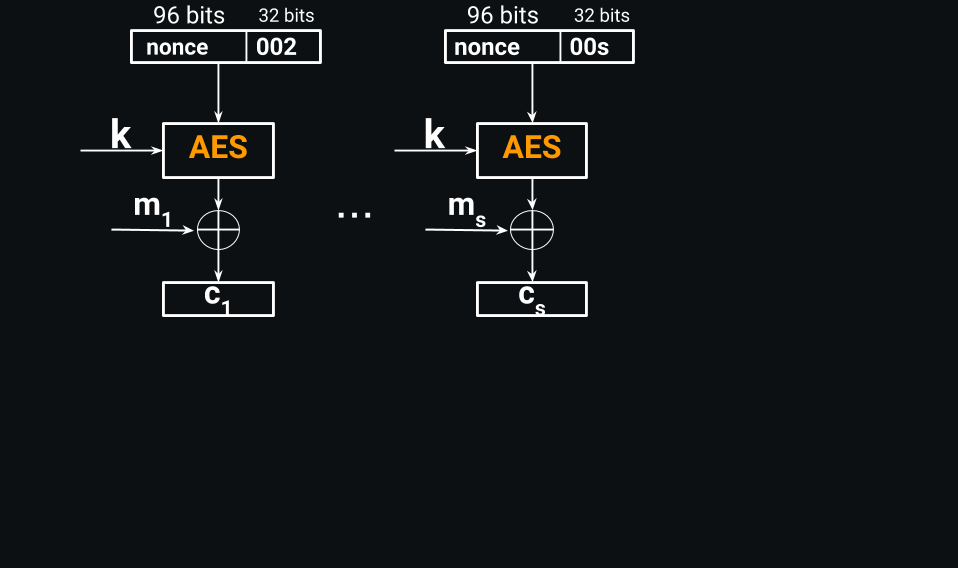
\includegraphics[width=\linewidth]{AES_GCM_AEAD_1}
%	\end{figure}
%}
%\only<2>
%{
%	\begin{figure}
%		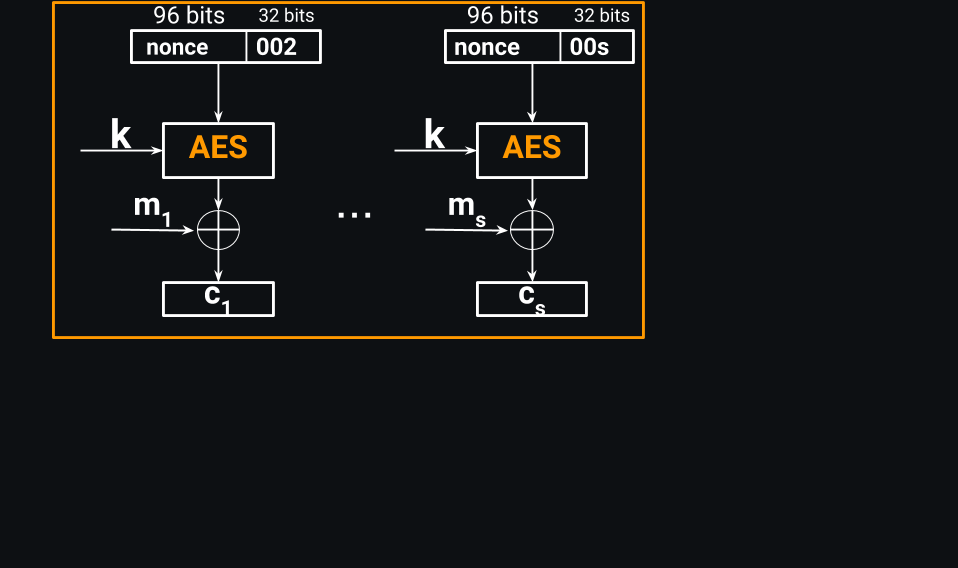
\includegraphics[width=\linewidth]{AES_GCM_AEAD_2}
%	\end{figure}
%}
%\only<3>
%{
%	\begin{figure}
%		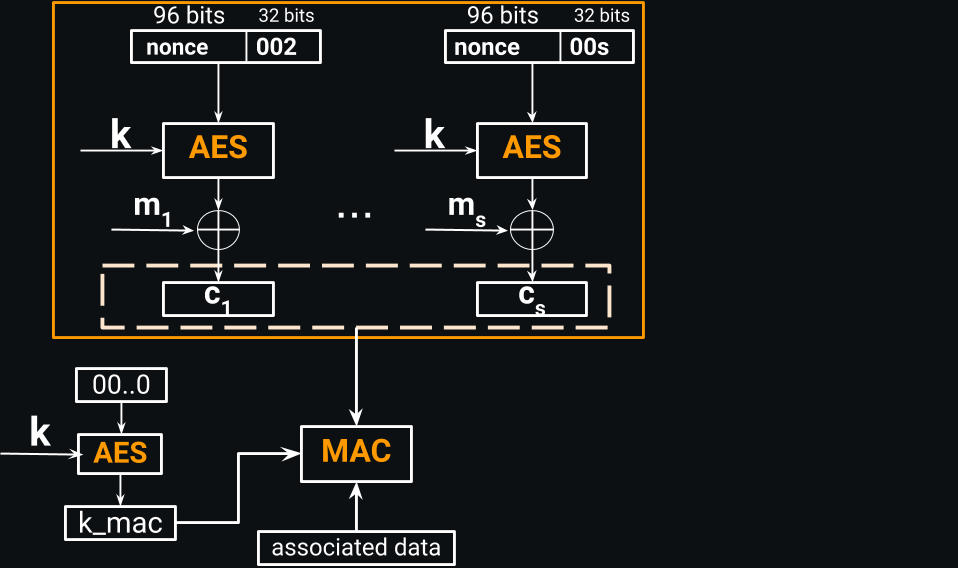
\includegraphics[width=\linewidth]{AES_GCM_AEAD_3}
%	\end{figure}
%}
%\only<4->
%{
%	\begin{figure}
%		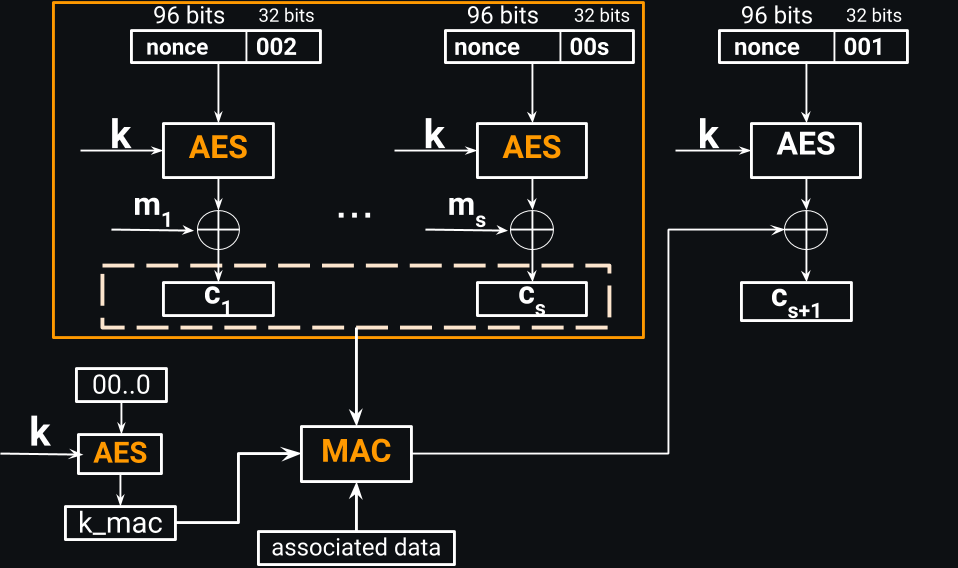
\includegraphics[width=\linewidth]{AES_GCM_AEAD_full}
%	\end{figure}
%}
%\only<5>
%{
%Output $(c_1, \ldots, c_s, c_{s+1})$
%}
%\end{frame}
%
%\begin{frame}{AES-GCM AEAD}
%\begin{figure}
%	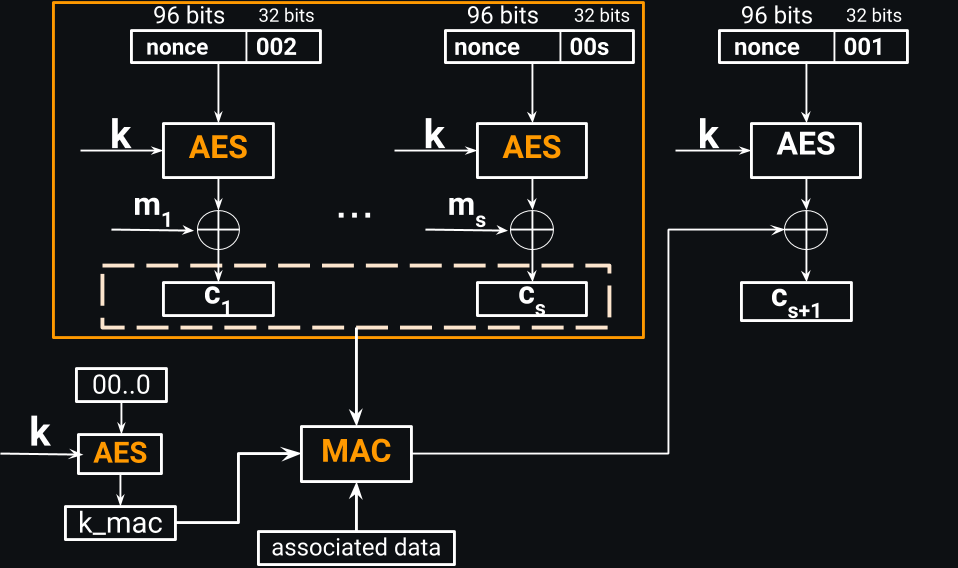
\includegraphics[width=0.7\linewidth]{AES_GCM_AEAD_full}
%\end{figure}
%
%\begin{itemize}
%	\item Uses just one key
%	\item MAC: GHASH (Galois Hash) - uses finite field arithmetic (fast)
%	\item Decryption: \\
%	1. Verifies MAC \\
%	2. $\Dec(c_1, \ldots, c_s)$
%\end{itemize}
%
%\end{frame}
%\begin{frame}{AEAD in TLS 1.3}
%	\LARGE
%	\begin{center}
%		\begin{tabular}{c c c }
%			\texttt{Browser}&  {\color{Orange}{Phase 1} Handshake}   & \texttt{Web server}  \\
%			& {\Large Asymmetric Encryption}  & \\ 
%			& {\Large Common keys are derived}  & \\ 
%			$k_{b\rightarrow s}$&  & $k_{b\rightarrow s}$\\ 
%			$k_{s\rightarrow b}$&  & $k_{s\rightarrow b}$ \pause \\ 
%			&  {\color{Orange}{Phase 2} TLS record protocol}   &  \\
%			& {\Large AEAD}  & \\ 
%		\end{tabular}
%	\end{center}
%\end{frame}
%
%\begin{frame}{TLS record protocol}
%\Large Data = $\left[m_1, \ldots, m_s\right]$
%\LARGE
%\begin{center}
%	\begin{tabular}{c c c }
%\texttt{Browser}&   & \texttt{Web server}  \\
%$k_{b\rightarrow s}$&  & $k_{b\rightarrow s}$\\ 
%$k_{s\rightarrow b}$&  & $k_{s\rightarrow b}$  \\ 
%$ctr_{b\rightarrow s}$&  & $ctr_{b\rightarrow s}$\\ 
%$ctr_{s\rightarrow b}$& {\large$\underbrace{
%		\left[
%		\texttt{Meta data} || \;
%		m_i \; || \;
%		\texttt{Nonce}
%		\right]}$}  & $ctr_{s\rightarrow b}$  \\ 
%\multicolumn{3}{c}{ $\xrightarrow{ \hspace{1em}  \Huge \text{AES-GCM-AEAD}(k_{b\rightarrow s}) \hspace{3.4em} }$  }  \pause \\
%$ctr_{b\rightarrow s}++$&  & $ctr_{b\rightarrow s}++$\\ 
%\end{tabular}
%\end{center}
%
%\pause 
%\vspace{10pt}
%\texttt{Meta data} includes: record on the phase (1 or 2), TLS Version, \texttt{len}$(c)$ \\
%Counters $ctr$ are used to prevent replay attacks
%
%\end{frame}
%
%\begin{frame}{Programming Assignment \# 5}
%\Large
%OpenSSL provides interfaces to GCM, CCM AEs via \texttt{EVP}\\[15pt]
%
%
%This PA:  to implement Encryption and Decryption Interfaces for any two Authenticated Encryption
%\begin{itemize}
%	\item GCM 
%	\item CCM 
%	\item ChaCha20-Poly1305
%\end{itemize}
%
%\vspace{10pt}
%See \url{https://wiki.openssl.org/index.php/EVP_Authenticated_Encryption_and_Decryption} for code
%
%
%\end{frame}

\end{document}
